\documentclass[a4paper, 11pt, showtrims]{memoir}
\semiisopage

\chapterstyle{veelo}


%% ALTERNATIBAK / ALTERNATIVAS
%\chapterstyle{default}
%\chapterstyle{bianchi}
%\chapterstyle{brotherton}
%\chapterstyle{demo2}
%\chapterstyle{ell}
%\chapterstyle{ger}
%\chapterstyle{wilsondob}

\pdfobjcompresslevel 0


%% INFORMAZIOA / INFORMACIÓN %%
\newcommand{\egilea}{Iker Bereziartua Sagarna}
\newcommand{\zuzendariak}{
	Zuzendaria 1 / Director(a) 1\\
	Zuzendaria 2 / Director(a) 2
}
\newcommand{\izenburua}{Evaluating the Impact of Network Topology on Backdoor Attacks in Decentralized Federated Learning}
\newcommand{\data}{\today}


%% BAKARRIK BAT DESKOMENTATU, GRADU AMAIERAKO LANA BADA. BESTELA, DENAK KOMENTATU%%
%% DESCOMENTAR SOLO UNO SI ES UN TRABAJO FIN DE GRADO. SINO, COMENTAR TODOS%%

%\newcommand{\ikasketak}{Informatika Ingeniaritzako Gradua}
%\newcommand{\ikasketak}{Grado en Ingeniería Informática}
%\newcommand{\ikasketak}{Degree in Informatics Engineering}
%\newcommand{\ikasketak}{Adimen Artifizialeko Gradua}
%\newcommand{\ikasketak}{Grado en Inteligencia Artificial}
\newcommand{\ikasketak}{Degree in Artificial Intelligence}


%% BAKARRIK BAT DESKOMENTATU, INGENIARITZA INFORMATIKAKOA BADA. BESTELA, DENAK KOMENTATU %%
%% DESCOMENTAR SOLO UNO SI ES EN INGENIERÍA INFORMÁTICA. SINO, COMENTAR TODOS %%

%\newcommand{\espezialitatea}{Konputazioa}
%\newcommand{\espezialitatea}{Computación}
%\newcommand{\espezialitatea}{Computing}
%\newcommand{\espezialitatea}{Software Ingeniaritza}
%\newcommand{\espezialitatea}{Ingeniería de Software}
%\newcommand{\espezialitatea}{Software Engineering}
%\newcommand{\espezialitatea}{Konputagailuen Ingeniaritza}
%\newcommand{\espezialitatea}{Ingeniería de Computadores}
%\newcommand{\espezialitatea}{Computer Engineering}

%% BAKARRIK BAT DESKOMENTATU MASTER AMAIERAKO LANA BADA. BESTELA, DENAK KOMENTATU%%
%% DESCOMENTAR SOLO UNO SI ES UN TRABAJO FIN DE MASTER. SINO, COMENTAR TODOS%%

%\newcommand{\ikasketak}{Máster Universitario en Ingeniería Computacional y Sistemas Inteligentes}
%\newcommand{\ikasketak}{Konputazio Ingeniaritza eta Sistema Adimentsuak Unibertsitate Masterra}

%% TESIENTZAKO KONFIGURATU
%\newcommand{\saila}{Department of Computer Science and Artificial Intelligence}
%\newcommand{\phdarloa}{Computer Science}
%% KOMENTATU A4 FORMATUAN ATERATZEKO, FORMATU TXIKIAGOAN AGERTZEKO 
%% GERO INPRIMATZEKO. MOZTEKO MARKAK IKUSTEKO GEHITU showtrims AUKERA
%% memoir KLASEAREN ARGUMENTUETAN
%\newcommand{\croppedsize}

%% DOKUMENTUAREN HIZKUNTZA / BAKARRIK BAT DESKOMENTATU %%
%% IDIOMA DEL DOCUMENTO / DESCOMENTAR SOLO UNO %%
%\newcommand{\euskaraz}{}
%\newcommand{\castellano}{}
\newcommand{\english}{}

\ifdefined\euskaraz
  \usepackage[eu]{ifcommands}
\else\ifdefined\english
  \usepackage[en]{ifcommands}
\else
  \usepackage[es]{ifcommands}
\fi\fi

\input config/macros



\title{\izenburua}
\author{\egilea}
\date{\data}


\begin{document}
 
%% AZALA BEREZIRIK BADUZU (PDF FORMATUAN), DESKOMENTATU%%
%% SI HAY UNA PORTADA ESPECIAL (EN PDF), DESCOMENTAR%%
	
%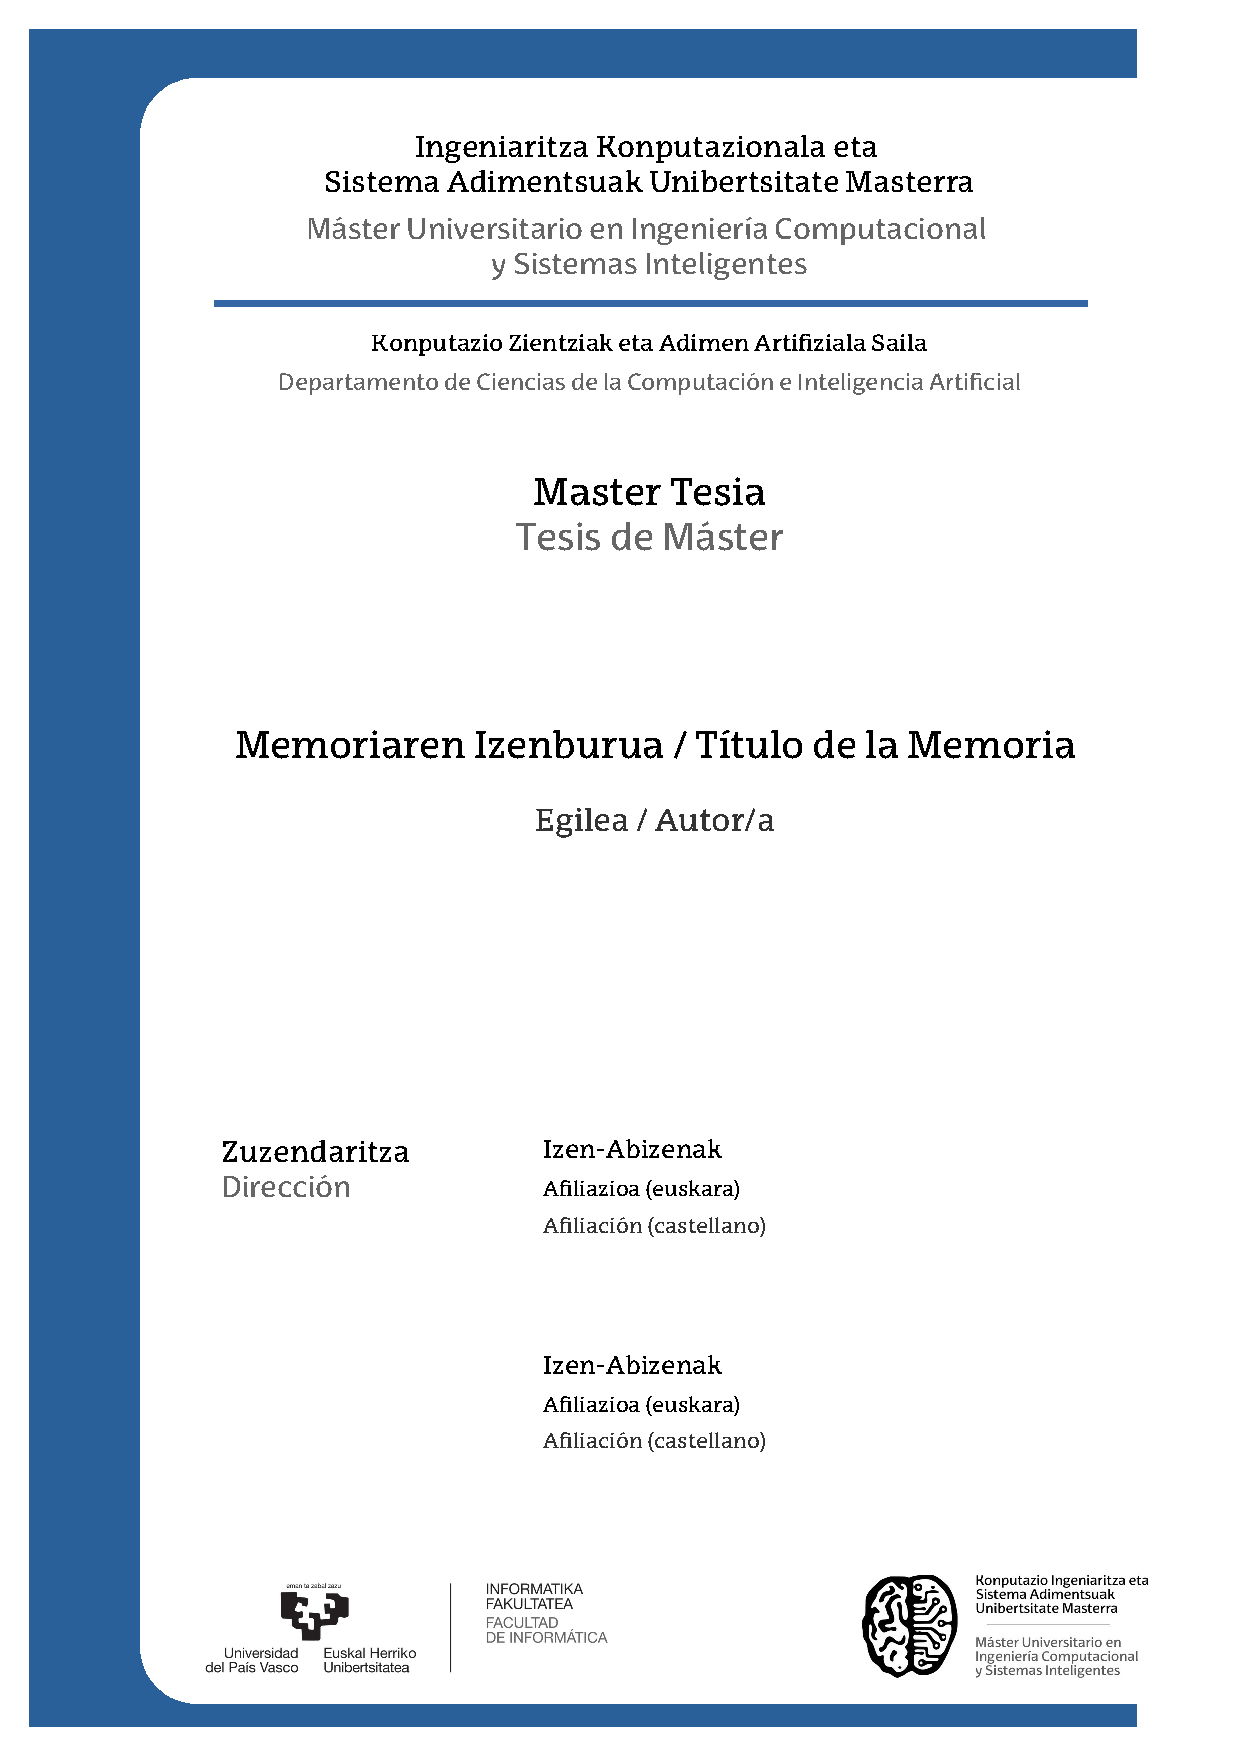
\includepdf[pages={1-}]{cover.pdf}
%\cleardoublepage
 
 
%% AUKERATU DAGOKIONA. AZALA BEREZIA GEHITUZ GERO, KOMENTATU DAITEKE, BETIERE HEMENGOAN AGERTZEN DEN INFORMAZIOA AGERTZEN BADA %%
%% SELECCIONA LA QUE CORRESPONDA. EN CASO DE TENER UNA PORTADA ESPECIAL SE PUEDE COMENTAR, SIEMPRE Y CUANDO DICHA PORTADA INCLUYA LA INFORMACIÓN QUE APARECE EN ESTA%%
 
%\input config/cover_informatika
\input config/cover_adimen_artifiziala
%\input config/cover_masterra
%\input config/cover_phd_dissertation
 
\cleardoublepage
\frontmatter
\aliaspagestyle{chapter}{plain}
\aliaspagestyle{cleared}{plain}
\pagestyle{plain}
\setcounter{page}{1}
 
%%%%%%%%%%%%%%%%%%%%%%%%%%%%%%%%
% ESKER ONAK / AGRADECIMIENTOS %
%%%%%%%%%%%%%%%%%%%%%%%%%%%%%%%%
 
%% KOMENTATU HIRU LERRO HAUEK ATALA NAHI EZ BADUZU
%% COMENTA ESTAS TRES LÍNEAS SI NO QUIERES ESTE APARTADO
\chapter*{Esker onak / Agradecimientos}
\input chapters/acknowledgements
\cleardoublepage
 
%%%%%%%%%%%%%%%%%%%%%%%
% LABURPENA / RESUMEN %
%%%%%%%%%%%%%%%%%%%%%%%
 
\chapter*{Laburpena / Resumen}
\input chapters/abstract
\cleardoublepage
 
\ifdefined\euskaraz
\chapter*{Garapen Jasangarrirako Helburuak} \label{ch:GJH}
\input chapters/GJH_ODS_SDG/GJH
\else\ifdefined\english
\chapter*{Sustainable Development Goals} \label{ch:SDG}
\input chapters/GJH_ODS_SDG/SDG
\else
\chapter*{Objetivos de Desarrollo Sostenible} \label{ch:ODS}
\input chapters/GJH_ODS_SDG/ODS
\fi\fi
 
\cleardoublepage
 
%%%%%%%%%%%%%%%%%%%%%%%%%%%%%%
% EDUKIEN ZERRENDA / ÍNIDCES %
%%%%%%%%%%%%%%%%%%%%%%%%%%%%%%
 
\openany
\pdfbookmark[1]{\contentsname}{toc}
\begin{KeepFromToc}
  \tableofcontents
\end{KeepFromToc}
\clearpage
\listoffigures
\clearpage
\listoftables
\clearpage
\listofalgorithms
\openright
 
%%%%%%%%%%%%%%%%%%%%%%
% EDUKIA / CONTENIDO %
%%%%%%%%%%%%%%%%%%%%%%
 
\cleardoublepage
\mainmatter
\pagestyle{ruled}
 
\chapter{Introduction} \label{ch:introduction}
\input chapters/Introduction 
\cleardoublepage

\chapter{Theoretical Framework} \label{ch:theoretical framewrk}
\input chapters/TheoreticalFramework
\cleardoublepage

\chapter{Threat Landscape in Decentralized Learning} \label{ch:threat landscape}
\input chapters/ThreatLandscapeInDecentralizedLearning 
\cleardoublepage

\chapter{Methodology} \label{ch:methodology}
\input chapters/Methodology 
\cleardoublepage

\chapter{Experimentation}
\label{ch:experimentation}
The main objective of this experimental setup is to explore the vulnerabilities explained previously, specifically backdoor attacks. By simulating a targeted backdoor attacks across different network structures, this research aims to understand how the lack of centralization affects the security of the learning process and how different communication topologies might naturally slow down or accelerate the spread of this type of attacks. All experiments were done using a custom Flower environment \cite{beutel2020flower}. The source code and configuration files used to reproduce all the experiments are publicly available at: https://github.com/IkerMardure/tfg-gossip-learning-backdoor/tree/master/GLow-master


\section{Evaluated Network Topologies} \label{sec:evaluated_topologies}

In Decentralized Federated Learning, the communication infrastructure is modeled mathematically as a graph $\mathcal{G} = (\mathcal{V}, \mathcal{E})$, where $\mathcal{V}$ represents the set of participating nodes (clients) and $\mathcal{E}$ represents the set of communication edges (links) between them \cite{palmieri2024impact}. Because nodes only aggregate models from their direct neighbors, the structural properties of $\mathcal{G}$ dictate the flow of parameters, the speed of global convergence, and the network's inherent resilience to malicious injections. 

To systematically evaluate these dynamics and establish a comprehensive baseline, decentralized networks were analyzed across a spectrum of connectivity, ranging from highly sparse to fully dense structures. The four foundational topologies evaluated in this research are visualized theoretically in Figure \ref{fig:topologies_theory} and defined as follows:

\begin{figure}[t]
    \centering
    % Primera Fila
    \subfloat[Fully Connected\label{fig:fc}]{%
        
\includegraphics[width=0.45\textwidth]{figures/fc_5_graph.png}%
    }\hfill
    \subfloat[Ring Topology\label{fig:ring}]{%
        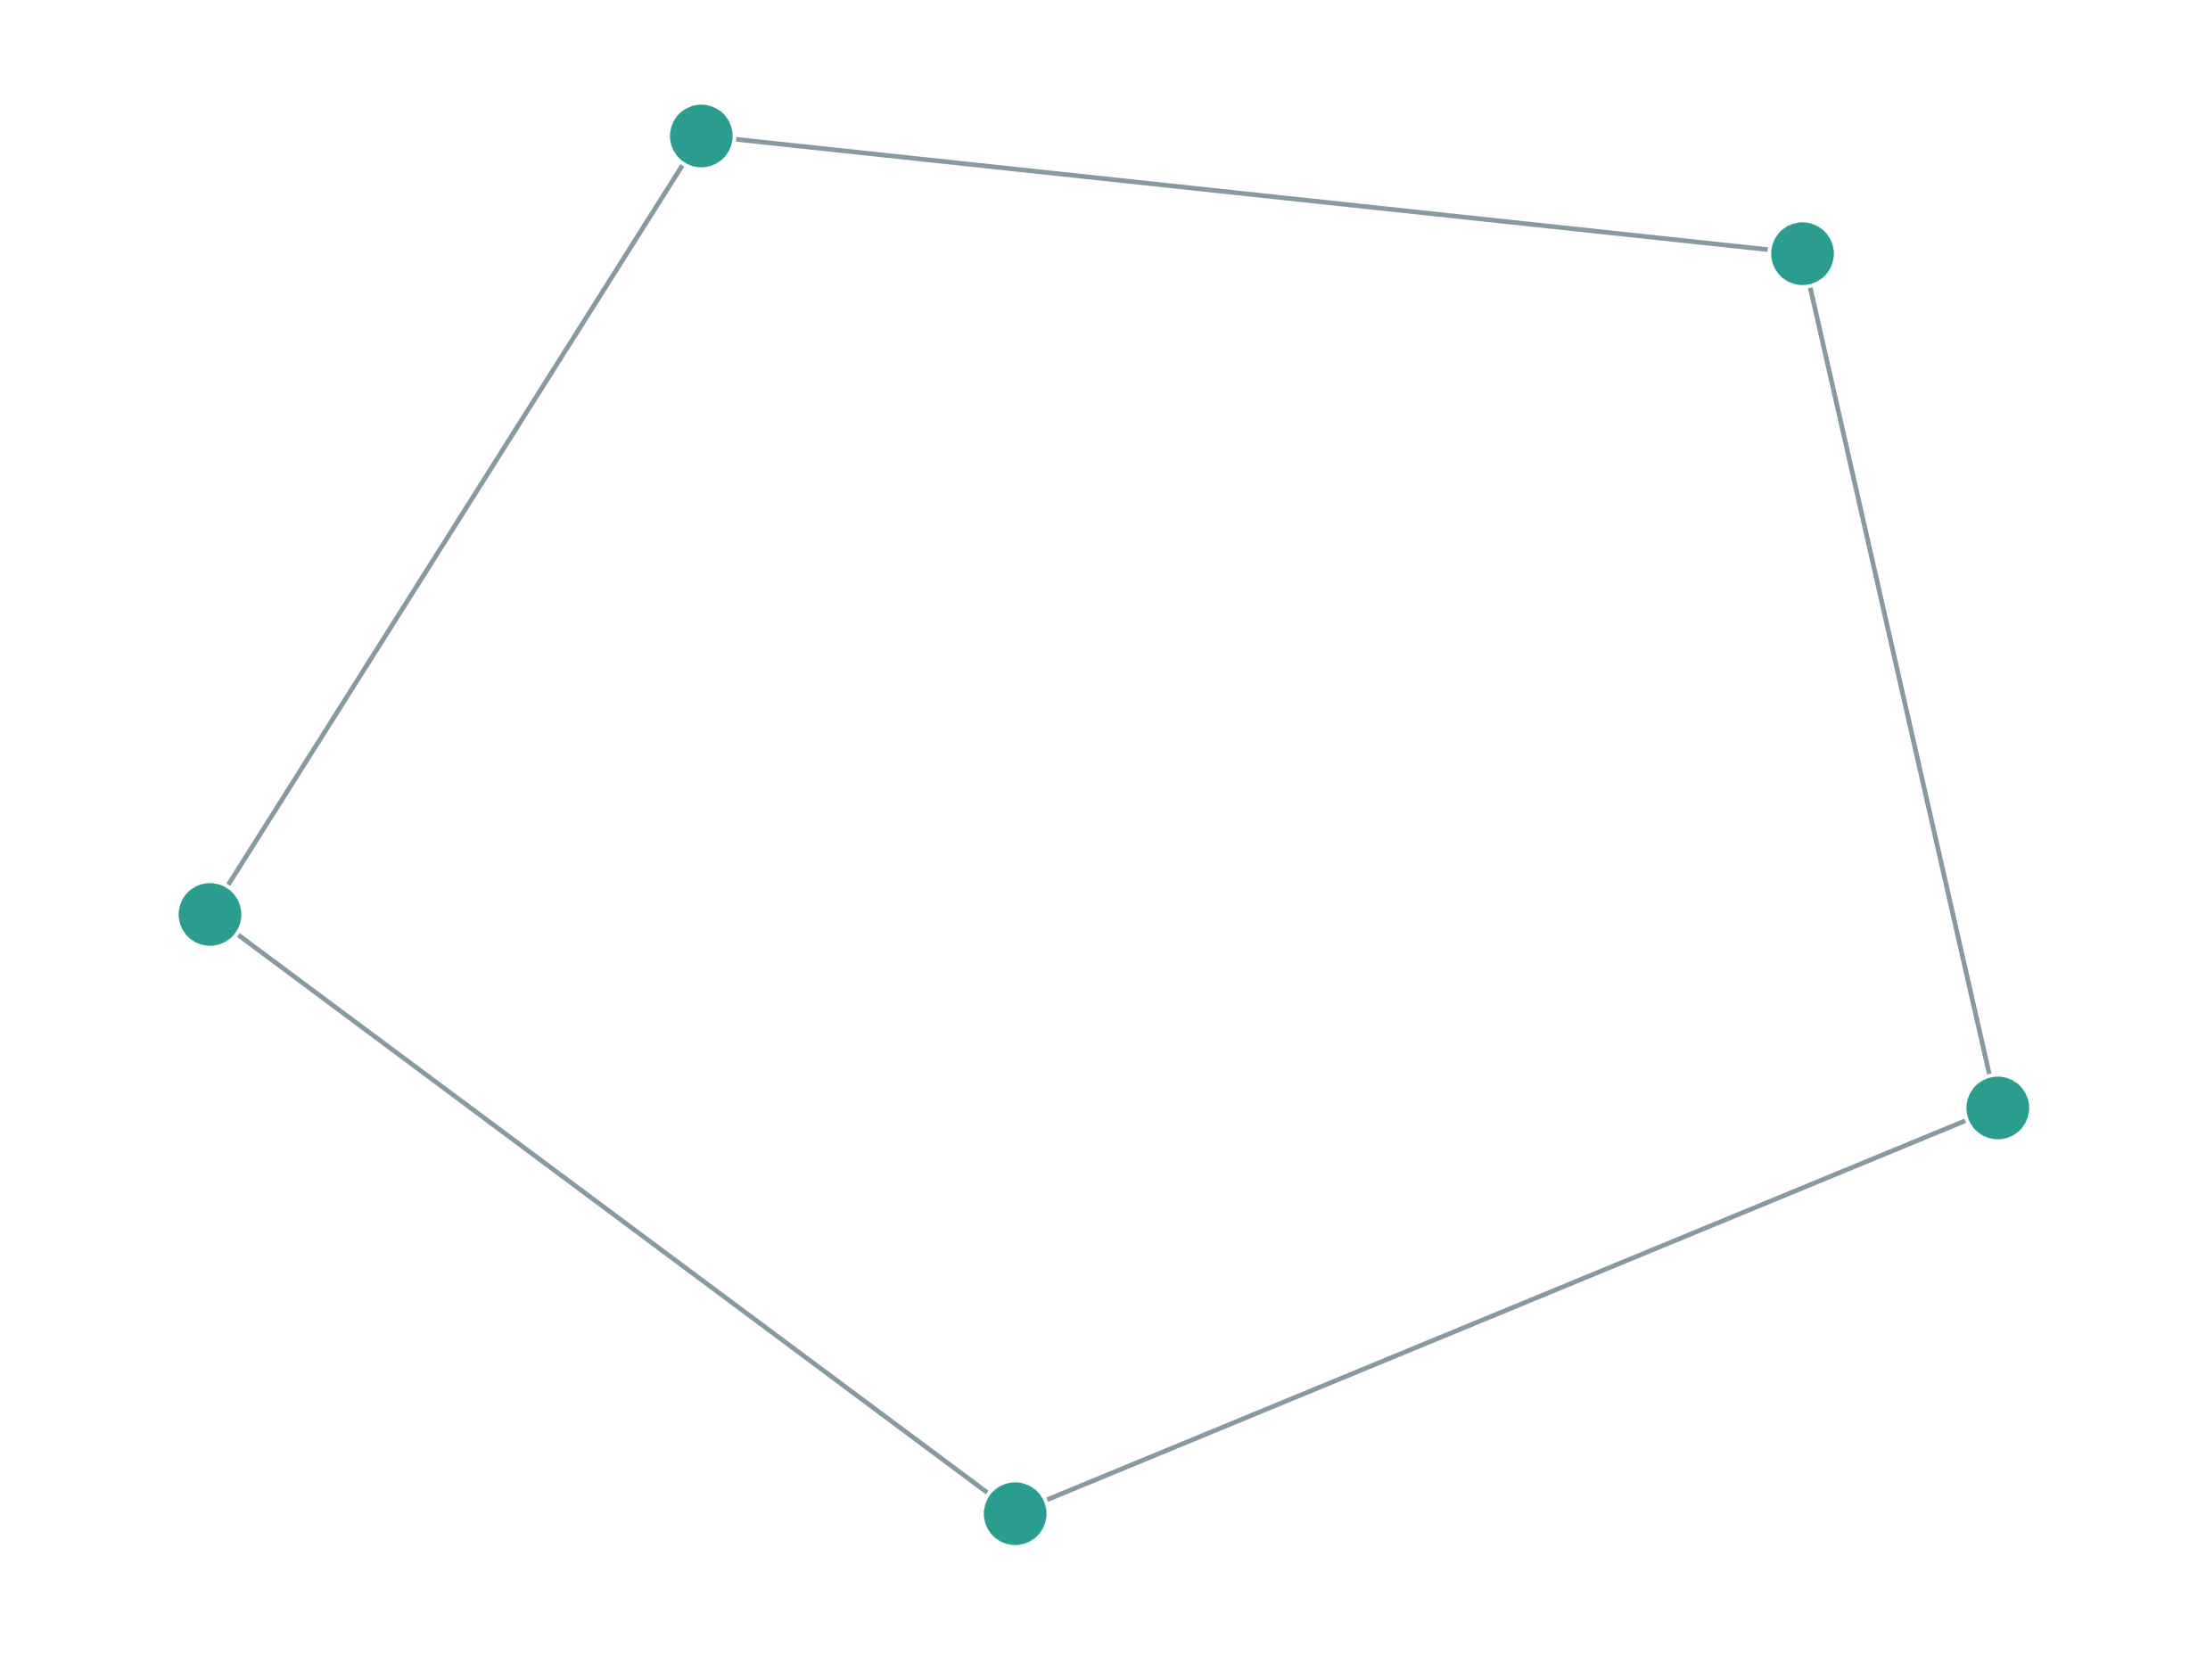
\includegraphics[width=0.45\textwidth]{figures/ring_5_graph.png}%
    }
    
    \vspace{1.5em}
    
    % Segunda Fila
    \subfloat[Star Topology\label{fig:star}]{%
        
\includegraphics[width=0.45\textwidth]{figures/star_5_graph.png}%
    }\hfill
    \subfloat[Stochastic Block Model\label{fig:sbm_theory}]{%
        
\includegraphics[width=0.45\textwidth]{figures/EC_8_graph.png}%
    }
    \caption{Theoretical visualization of the four network topologies evaluated in this study.}
    \label{fig:topologies_theory}
\end{figure}

\begin{itemize}
    \item \textbf{Fully Connected Topology:} A Fully Connected (FC) or complete graph is a topology where every node shares a direct edge with every other node in the network (Figure \ref{fig:fc}). The topological distance (network diameter) is strictly one hop. This structure represents the maximum possible density in a peer-to-peer network, allowing for immediate, unimpeded dissemination of knowledge. In these experiments, it is expected that denser networks will accelerate the backdoor attack due to direct peer-to-peer exposure. 
    
    \item \textbf{Ring Topology:} A Ring topology represents a highly sparse, constrained network configuration (Figure \ref{fig:ring}). Each node is connected to exactly two immediate neighbors, forming a single closed loop where information travels slowly \cite{giaretta2019gossip}. Because there are no cross-network shortcuts, information must propagate sequentially. This structural bottleneck significantly delays the spread of both legitimate knowledge and potential adversarial payloads, naturally delaying the backdoor infection.
    
    \item \textbf{Star Topology:} A Star topology is characterized by a single central node (the hub) connected to multiple peripheral nodes, while the peripheral nodes remain completely isolated from one another (Figure \ref{fig:star}). In a DFL context, this localizes the centralized FL paradigm. The central hub acts as a powerful aggregator, continuously absorbing and averaging updates from all peripherals to create a strong "consensus wall" capable of diluting anomalous updates originating from the periphery.
    
    \item \textbf{Stochastic Block Model (SBM):} Real-world decentralized networks rarely follow perfectly uniform shapes; instead, they naturally form communities. To mathematically capture this, Holland et al. \cite{holland1983stochastic} introduced the Stochastic Block Model, where nodes are partitioned into distinct blocks with a higher probability of intra-community edges than inter-community edges. This creates dense local clusters connected by sparse "gateway" links, trapping information in local echo chambers.
\end{itemize}

\textbf{Deterministic SBM Implementation}\\
It is important to note that while the theoretical Stochastic Block Model \cite{holland1983stochastic} is a probabilistic framework relying on random edge generation, our experimental methodology requires a controlled, deterministic environment to accurately isolate and measure the attack's propagation. 

Therefore, rather than using random connections, we implemented a strictly deterministic community-based structure that mathematically mirrors the core characteristics of an SBM. As shown in Figure \ref{fig:sbm_setup}, the implemented network consists of two distinct communities containing three nodes each. Within each community, the nodes are fully connected to ensure rapid local consensus. However, the two communities are bridged by exactly one fixed gateway connection. This deterministic design guarantees that if a malicious node operates within one community, the gateway acts as a strict, quantifiable bottleneck, actively hindering the infection's progression to the external community.

\begin{figure}[t]
    \centering
    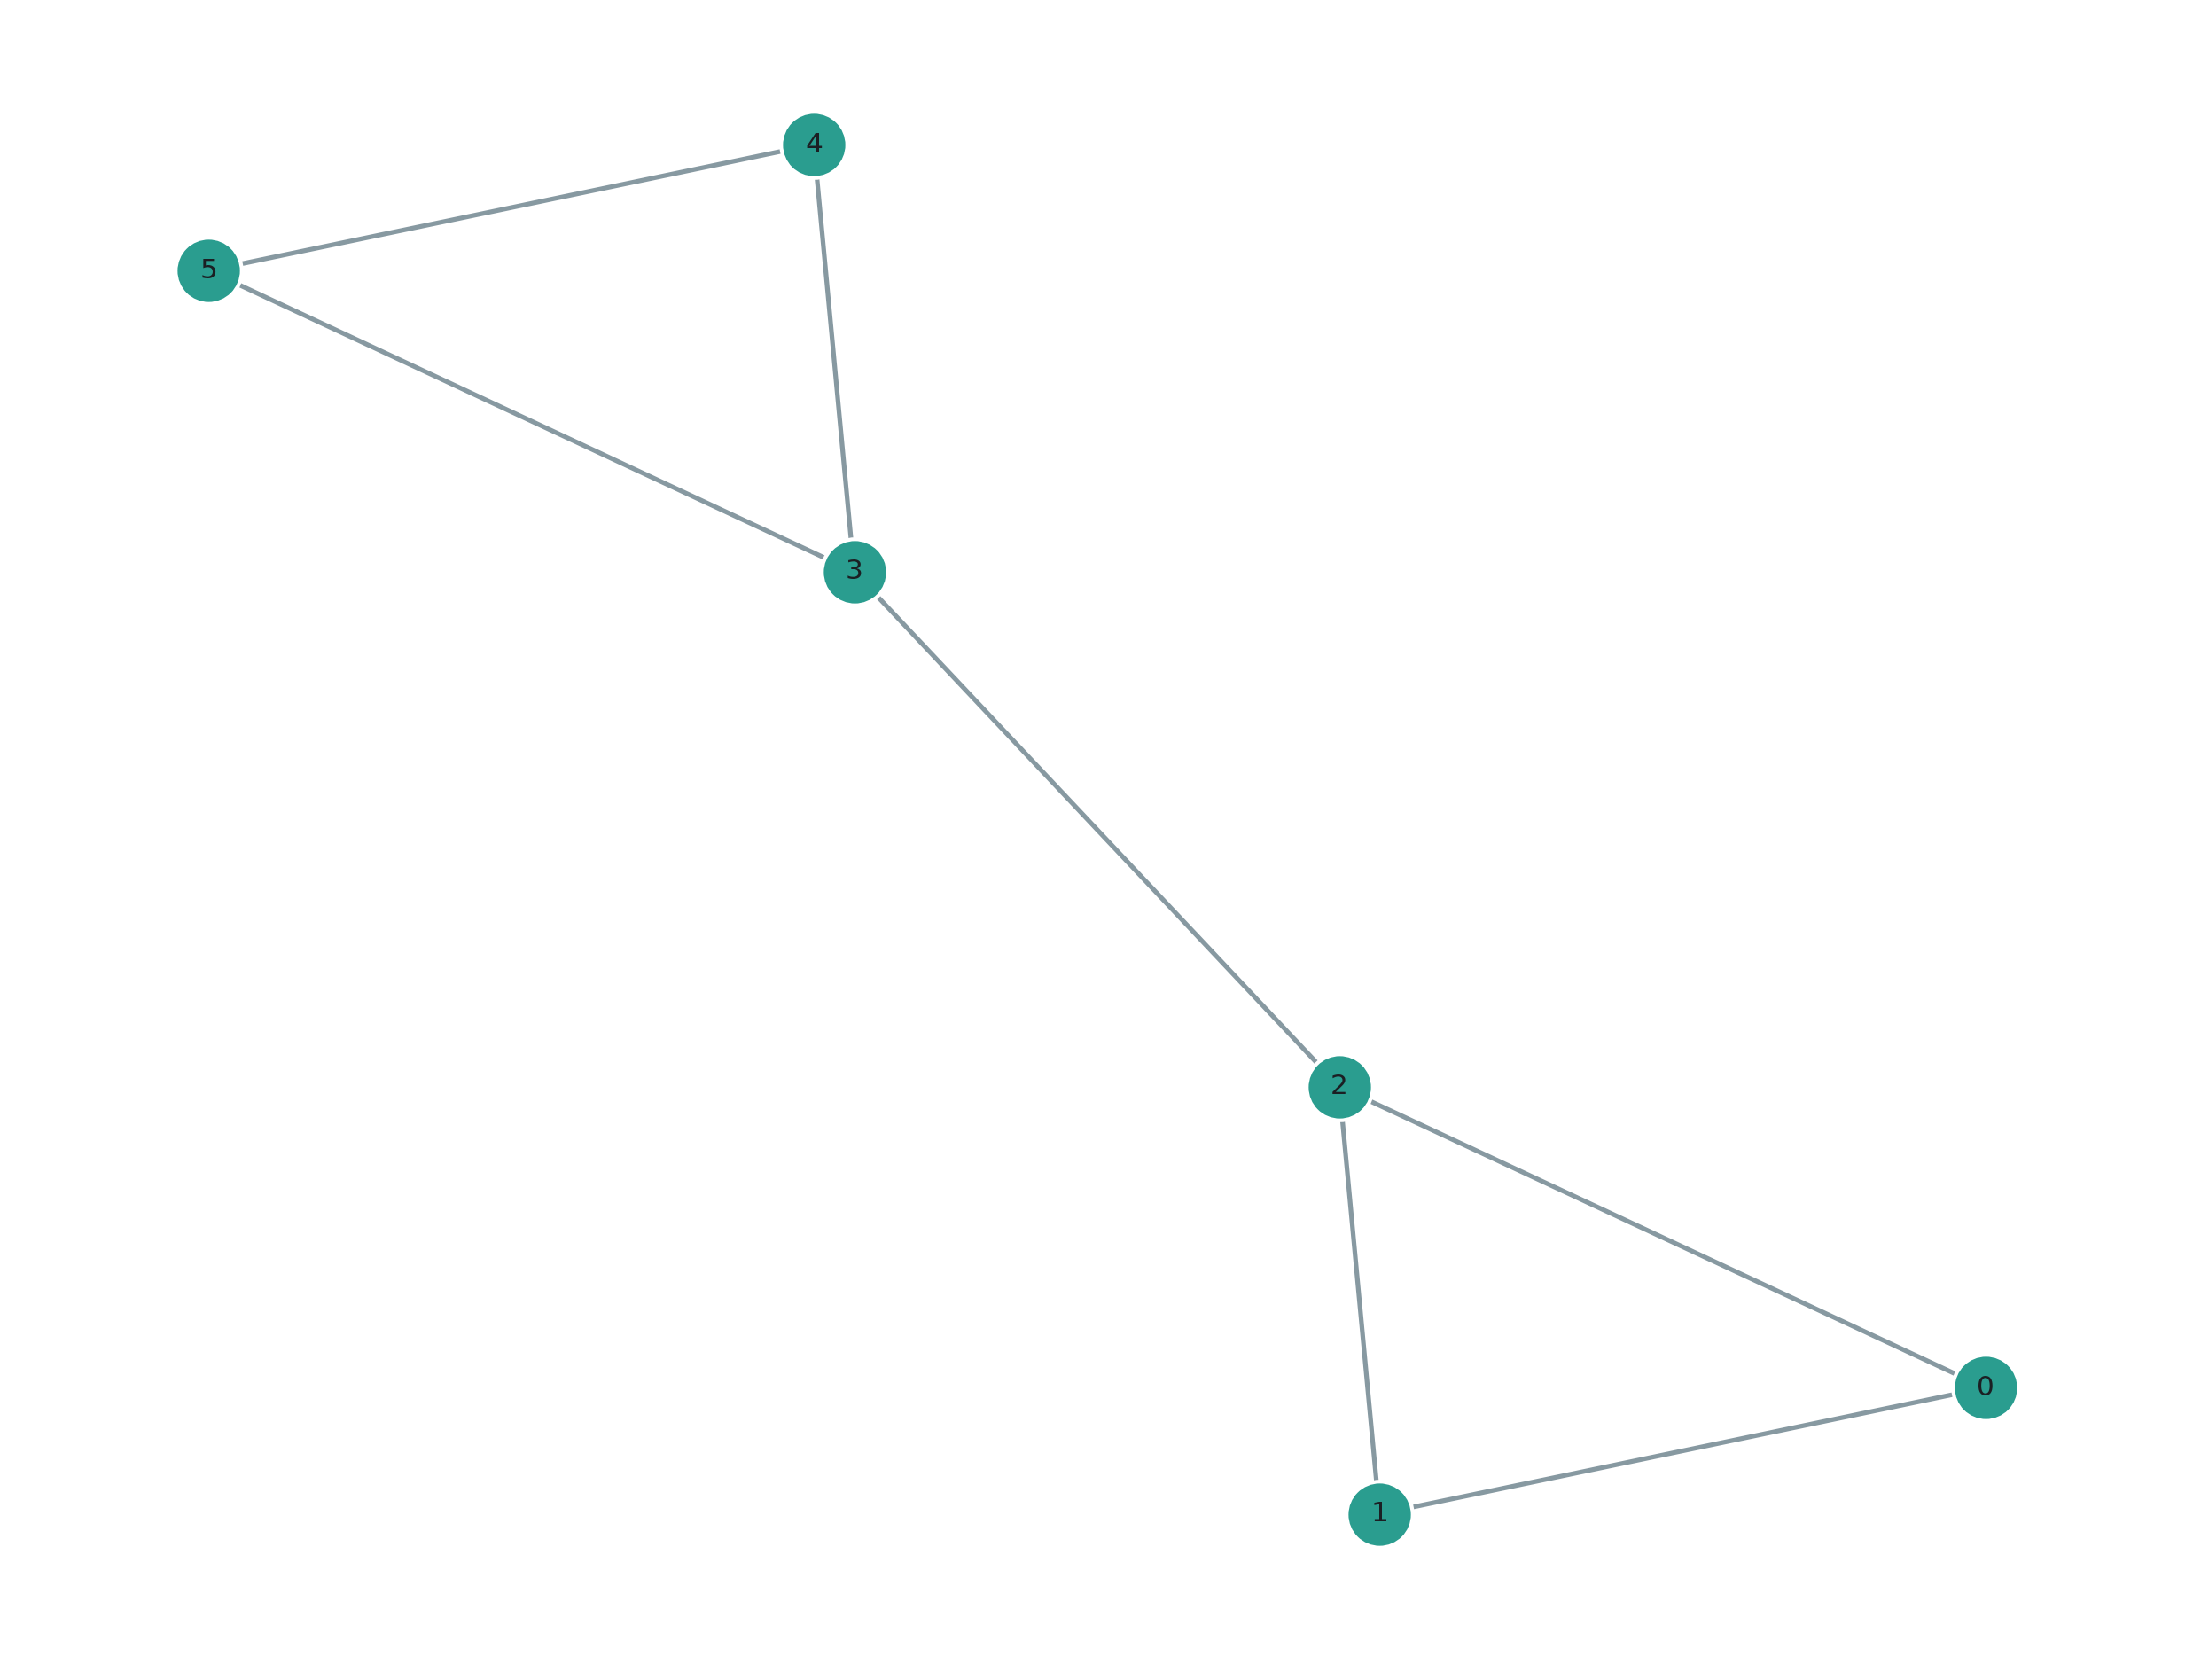
\includegraphics[width=0.6\textwidth]{figures/EC_6_graph.png}
    \caption{Experimental setup for the deterministic Stochastic Block Model (SBM). The network is strictly divided into Community A and Community B, connected via a single gateway. The designated malicious node (Client 1) is placed within Community A.}
    \label{fig:sbm_setup}
\end{figure}


\section{Experimental Setup: Dataset, Architecture, and Metrics}
The primary experiment was conducted using the MNIST dataset \cite{lecun1998gradient}. To align with the architectural requirements of the model, all the images were resized to 32x32 pixels. The classification task was constrained to a subset of 5 classes, primarly to lower computational cost. To establish a controlled and uniform baseline for the experiments, the dataset was partitioned in an Independent and Identically Distributed (IID) manner among the clients. This ensures that each node starts with a statistically similar subset of the data.

A modified $LeNet$ \cite{lecun1998gradient} architecture was used as the local model across all nodes. The network is composed of three convolutional layers of 16, 32 and 64 filters, repectively, each with $3 \times 3$ kernels and a padding of 1. Each convolutional operation is followed by a ReLU activation function and a $2 \times 2$ Max Pooling operation. The resulting feature maps are processed through two fully connecyed layers, the first containing 128 units and the last one containing as much units as the classes used, in this case 5. 
Furthermore, a dropout layer with a $0.2$ probability was inserted prior to the final classification layer to mitigate overfitting during the training.
The global training process spanned 20 communication rounds, during which the active client performed local training for 2 epochs using a batch size of 128. The local optimization was handled by the Adam optimizer \cite{kingma2014adam} with a learning rate set to 0.0001 and a momentum of 0.9.

To evaluate the attack, two measurements were used: Clean Accuracy and Attack Success Rate (ASR). Clean Accuracy measures how well each node classifies the unmodified test data, which is critical for observing how undetectable the attack remains during normal operation. In contrast, the ASR is calculated using modified test data to indicate the spread and effectiveness of the attack through the network.

\subsection{Simulation Constraints and Execution Flow}

While the theoretical framework of Gossip Learning assumes parallel execution across all participating nodes (as outlined in Algorithm \ref{alg:gossip_learning}), simulating such a decentralized network on centralized hardware introduces practical implementation constraints. 

In our experimental setup using the Flower framework, the local training phases for the clients were executed sequentially within each communication round due to computational resource limits. However, from a logical standpoint, the network state is frozen during the training phase, and parameter exchanges are only aggregated at the end of each discrete round. This effectively simulates a synchronous, parallel execution environment. Because the primary focus of this research is the structural propagation of malicious weights through specific graph topologies rather than evaluating computational time delays or asynchronous race condition, this sequential simulation accurately preserves the integrity of the topological vulnerabilities being evaluated.
\cleardoublepage

\chapter{Experimental Results and Discussion} \label{ch:results}
\input chapters/ExperimentalResultsAndDiscussion 
\cleardoublepage

\chapter{Conclusions and Future Work}\label{ch:conclusions}
\input chapters/Conclusions
\cleardoublepage
 
%%%%%%%%%%%%%%%%%%%%%%%%%%%%
%% ERANSKINAK / APENDICES %%
%%%%%%%%%%%%%%%%%%%%%%%%%%%%
 
\addappheadtotoc
\appendix
 
\ifdefined\euskaraz
\chapter{AA sortzailearen erabilera deklarazioa} \label{ch:deklarazioa}
\input chapters/appendix/deklarazioa
\else\ifdefined\english
\chapter{Declaration of use of generative AI} \label{ch:declaration}
\input chapters/declaration
\else
\chapter{Declaración del uso de IA Generativa} \label{ch:declaracion}
\input chapters/appendix/declaracion
\fi\fi
 
 
%%%%%%%%%%%%%%%%%%
%% BIBLIOGRAFIA %%
%%%%%%%%%%%%%%%%%%
\bibliographystyle{unsrt}
\bibliography{erreferentziak}

 
\end{document}
